\section{Analysis of Gathered Data}

\subsection{Literature Review}

To find the root course of fault in a distributed system, three components are required: instrumentation, anomaly detection, and root course localization. A literature review was conducted on each of the components to derive the requirements needed to build an automated root course analysis platform.

% To find the root course of fault in a distributed system, three components are required, instrumentation, anomaly detection, and root course localization. Those three must work together to give a final prediction. From these three, anomaly detection has a lot of possible pathways to approach the problem. This is mainly due to anomaly detection being a broad topic that isn't limited to cloud computing. For the sake of this project using a semi-supervised technique with a convolutional autoencoder network seemed like the idle approach since those networks are lightweight and more reliable when it comes to generalizing. For instrumentation use of a Linux kernel feature called \ac{ebpf} seemed the current treading method due to it being very lightweight and not requiring any code changes to the existing system. Finally for the root course localization almost all the published work used graphed based method one way or another due to the nature of the problem being always dynamic. So the author decide to rely on a weighted graph to find a possible root course after an anomaly is detected.

\begin{longtable}{|p{105mm}|p{50mm}|}
    \hline
    \textbf{Finding} &
    \textbf{Citation} \\ \hline
    
    \ac{ebpf} is a modern, low overhead technique to extract telemetry by tracing Linux kernel calls. &
    \cite{LKMLIngo52:online} \\ \hline
    
    To find the root course of a fault in a distributed system, three components are required: instrumentation, anomaly detection, and root course localization. &
    \cite{wu2020microrca} \\ \hline
    
    Unsupervised learning algorithms excel at identifying unknown pattern. &
    \cite{silver2017mastering}, \cite{kumarage2018anomaly}, \cite{khoshnevisan2019rsm} \\ \hline
    Convolutional autoencoder network will give the best performance to resources required ratio when it comes to detecting anomalies. &
    \cite{zhang2019deep}, \cite{khoshnevisan2019rsm} \\ \hline
    
    Root course could be identified by weighting anomaly scores in directed graphs. &
    \cite{samir2019dla}, \cite{wu2020microrca}, \cite{ma2020automap}, \cite{meng2020localizing} \\ \hline
    There isn’t a common benchmarking or testing platform to test root causes of finding algorithms. &
    \cite{wu2020microrca}, \cite{soldani2021anomaly} \\ \hline
    
    Kubernetes is the go to method to manage distributed systems &
    \cite{CloudNat36:online} \\ \hline

    \caption{Requirements derived from literature review (self-composed)}
    
\end{longtable}

\subsection{Interviews}

A set of qualitative interviews was conducted to gather external feedback and opinion about the project and proposed system. For this, a senior production engineer, a Senior software engineer, a software engineer, and a trainee DevOps engineer were interviewed. The following table breaks down themes that were emerged after analyzing the transcript and findings based on that.
\newpage
\begin{longtable}{|p{30mm}|p{61mm}|p{60mm}|}
    \hline
    \textbf{Theme} &
    \textbf{Review} &
    \textbf{Evidence} \\ \hline
    
    Finding the root cause &
    Almost all the interviewees agreed that whenever there is an outage, it’s a cumbersome task to find the root course of that outage. Having a system that makes this experience even slightly better would have huge implications. &
    "I mean so often, sometimes it's identifying what the problem even is.” - Matthias Rampke (00:31:39)
    \newline
    \newline
    “I mean, figuring out the problem is always hard because you're under stress.” - Jacob Payne (00:23:27)
    \\ \hline

    
    
    ML for RCA &
    This is a bit of a gray area. One of the experts I interviewed said he had a long history of working with time series forecasting and results are generally mediocre due to the sheer number of external factors. But since this is a closed system results may vary. &
    “Ideally it helps me understand why the AI thinks this service is the problem.” \newline- Matthias Rampke (00:35:51)
    \newline
    \newline
    “It could also be useful if it could trace outage implications.” \newline- Jonathan Reiter \\ \hline
    
    
    Kubernetes &
    Almost all the technical experts I have talked to agreed-upon Kubernetes is the way to manage distributed systems in the modern era and building this system tailor-made to Kubernetes was a wise choice. &
    “I think there's been a lot of, uh, or an interesting shift that's been happening in this and it's sort of driven by Kubernetes.” \newline- Matthias Rampke (00:25:11)
    \newline
    “I mean, in the last five years, obviously Kubernetes blew up. That's been huge for the Dev-Ops community.” \newline- Jacob Payne (00:16:38) \\ \hline
        
    
    Service Meshes &
    Experts have a “love-hate” relationship with Service Meshes. Service Meshes offers a lot of utility functions and useful data for debugging. But at the same time, they require a lot of resources to configure and maintain. &
    “Going through a service mesh is a big investment, so I think there is a space for a smaller thing.” \newline- Matthias Rampke (00:05:04) \\ \hline
    
    Proposed Architecture &
    During interviews, the author showed the Alpha version of the product along with the high-level system diagram, and all the interviewees were impressed by it and excited to get their hand on the final product. &
    “I'm really looking forward to seeing it in action.”  \newline- Matthias Rampke (00:11:10)
    \newline
    \newline
    % “That's me, I think that's a lot of work, even for a capstone project to be on.” \newline- Jonathan Reiter (00:13:56)
    % \newline
    % \newline
    “I can tell you the project as it is right now has value and if you can get an MVP out there that can be installed as a side car, that's going to be huge.” \newline- Jacob Payne (00:36:09) \\ \hline

\caption{Inductive thematic analysis of interviews (self-composed)}
\end{longtable}

\subsection{Self-evaluation}



\begin{longtable}{|p{50mm}|p{105mm}|}
    \hline
    \textbf{Criteria} &
    \textbf{Finding} \\ \hline

    Ways to integrate with Kubernetes &
    There are two main ways to implement a system that interfaces with Kubernetes. From those creating standalone services that talk to Kubernetes API is the most straightforward method. But during Google Summer of Code 2021, the author worked on a project which uses a Kubernetes operator framework which is used to extend the functionality of Kubernetes. After evaluating both options it was decided to rely on the Kubernetes operator framework to build the controller for this project since it's a proven and reliable method to build services that interface with Kubernetes \citep{Introduc93:online}. \\ \hline

    Telemetry extraction method &
    Service meshes are currently the most common way of extracting telemetry but there is a huge focus on \ac{ebpf} related products due to it’s efficiency. \\ \hline

    New trends in DevOps &
    From CI/CD to GitOps, DevOps engineers are trying to automate everything that can be automated to minimize the human errors \citep{CloudNat36:online}. \\ \hline

    Case studies on recent high profile outages &
    Few months ago Microsoft experienced a global outage that took more than 24 hours to fully recover from. This waas due to a single bad update to one of their authentication systems \citep{Microsof81:online}. \\ \hline
    
    \caption{Requirements derived from self-evaluation (self-composed)}
\end{longtable}

% During the Self-evaluation of the existing system, it was made clear using \ac{ebpf} as the instrumentation technique has many benefits which range from very low overhead to fast and easier deployment but It comes with a few cons as well. The most notable example of this is the reliability of the collected data. Since \ac{ebpf} tracing works in lower of the TCP stack, there is a higher chance for corrupted data when compared to application layer level tracing which has all the bad packets filtered out. Still, the data points needed for this system like request rate can be calculated with good accuracy.

% Another reoccurring factor that was identified during this process was the use of Kubernetes. According to a recent survey done by Cloud Native Computing Foundation, 91\% of respondents stated they rely on Kubernetes to manage their container infrastructure \citep{CloudNat36:online}. So building the proposed system tailor-made for Kubernetes would reap the maximum benefit.

\subsection{Brainstorming}

\begin{longtable}{|p{50mm}|p{105mm}|}
    \hline
    \textbf{Criteria} &
    \textbf{Finding} \\ \hline

    Best way to detect anomalies &
    Learning objective of an autoencoder is given X input, Output X. Even though this doesn’t make sense as it is, this process allows the network to deeply understand the underlying function of the given data distribution. So after training at right conditions the model can output a value very close to input resulting in low reconstruction loss. But if the input data is something the model hasn’t seen during the training process (novel anomaly) model will produce a higher reconstruction loss. This could be used as a signal to identify the health of service. \\ \hline

    \caption{Requirements derived from brainstorming (self-composed)}
\end{longtable}

\subsection{Prototyping}

At the start of this project, a simple Proof of Concept (POC) was developed to understand the feasibility of the project. The experiment started with taking a Sine function and concatenating it with a noise function to create a variating data sequence. This was done to emulate service metrics in a small and easy-to-understand way. After that, the author created a simple encoder-decoder network which was tasked with giving an input sequence of 0 to n to predict the n to n+10 on the sequence. Figure \ref{fig:poc-autoencoder}shows the results of the experiment. The blue line shows the input given to the network while the green shows the ground truth results. Finally, the orange line is the model that predicts how the metric should be in any given time step. Notice there is a sudden dip around t=80, it's an artificially injected anomaly that isn't present in the training dataset and due to that, there is a clear difference between expected the current readings from the metric. The author's idea was to use this difference to find anomalies in real-time metrics. Even though this worked well for small-scale prototypes the author found that this doesn't translate to highly noisy sequences patterns found in production servers but this could be used as the entry point to a more robust solution. Refer to the Appendix \ref{appendix:poc-results} to read more about this experiment.

\begin{figure}[H]
    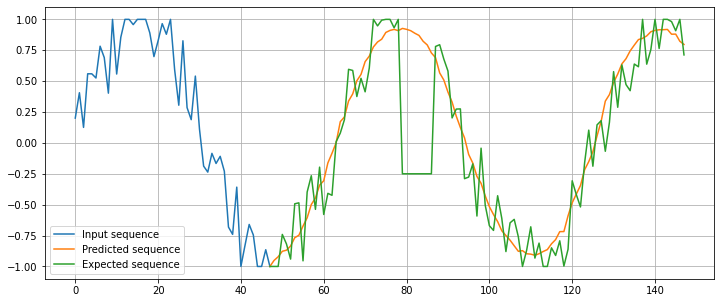
\includegraphics[width=14cm]{assets/requirement-specification/poc-autoencoder.png}
    \caption{The result from the proof of concept (self-composed)}
    \label{fig:poc-autoencoder}
\end{figure}
